
%
% Chapter 2
%

\chapter{BACKGROUND}
\label{chap:backgound}
This chapter gives a brief summary of related research on spectrum sharing, software defined radio (SDR) tools, the DARPA Spectrum Challenge, and the physical-layer foundation for radio designs.


\section{Related Research on Spectrum Sharing}

Game theory applications of wireless networks from a layered perspective are summarized in \cite{DimitrisECharilasAthanasiosDPanagopoulos:2010}, which discusses game theory in the physical layer, data link layer, network layer and transport layer. In physical layer game theory, power control, spectrum allocation, multiple-input multiple output (MIMO) systems and cooperative communications are highlighted.

A cooperative game for distributed spectrum sharing is studied in \cite {JuanESurisLuizADaSilvaZhuHanandAllenBMacKenzie2007}. According to this model, the available bandwidth is divided equally into multiple channels. Each transmitter can transmit in any combination of channels at any time and can set its transmit power on each channel. Receiver nodes are not considered in the game. A distributed algorithm based on the Nash Bargaining Solution is proposed. However, some practical issues, such as synchronization and feedback between the transmitter and receiver, are not considered.

Power control for spectrum sharing in an unlicensed band, in which multiple systems coexist and interfere with each other, is studied in \cite{REtkinandAParekhandDTse2007}. Consider an $M$-user Gaussian interference channel in discrete time. From an information-theoretic perspective, the best power control strategy for a given system in the competitive game for each user is to spread its available power over the entire bandwidth using the water filling method. This solution assumes that the users can accurately estimate the interference environment in which they are operating.

This thesis takes inspiration from these theoretical works, but specifically addresses important mechanisms for synchronization, feedback, and learning the interference environment.



\section{Software-Defined Radio (SDR) Tools}
Our radio is implemented with the GNU Radio 3.7.2 software \cite{GNURadio} and the USRP N210 hardware from Ettus Research \cite{EttusResearch}. GNU Radio is a free and open-source software development toolkit that provides signal processing blocks to implement software radios. It can be used with external RF hardware to create software-defined radios, or without hardware in a simulation-like environment. GNU Radio applications are written in C++ and Python. The signal processing blocks are implemented in C++, which can then be connected together in Python to form a flow graph to process data in a streaming fashion.
\begin{figure}[tpb]
  \begin{center}
    \centerline{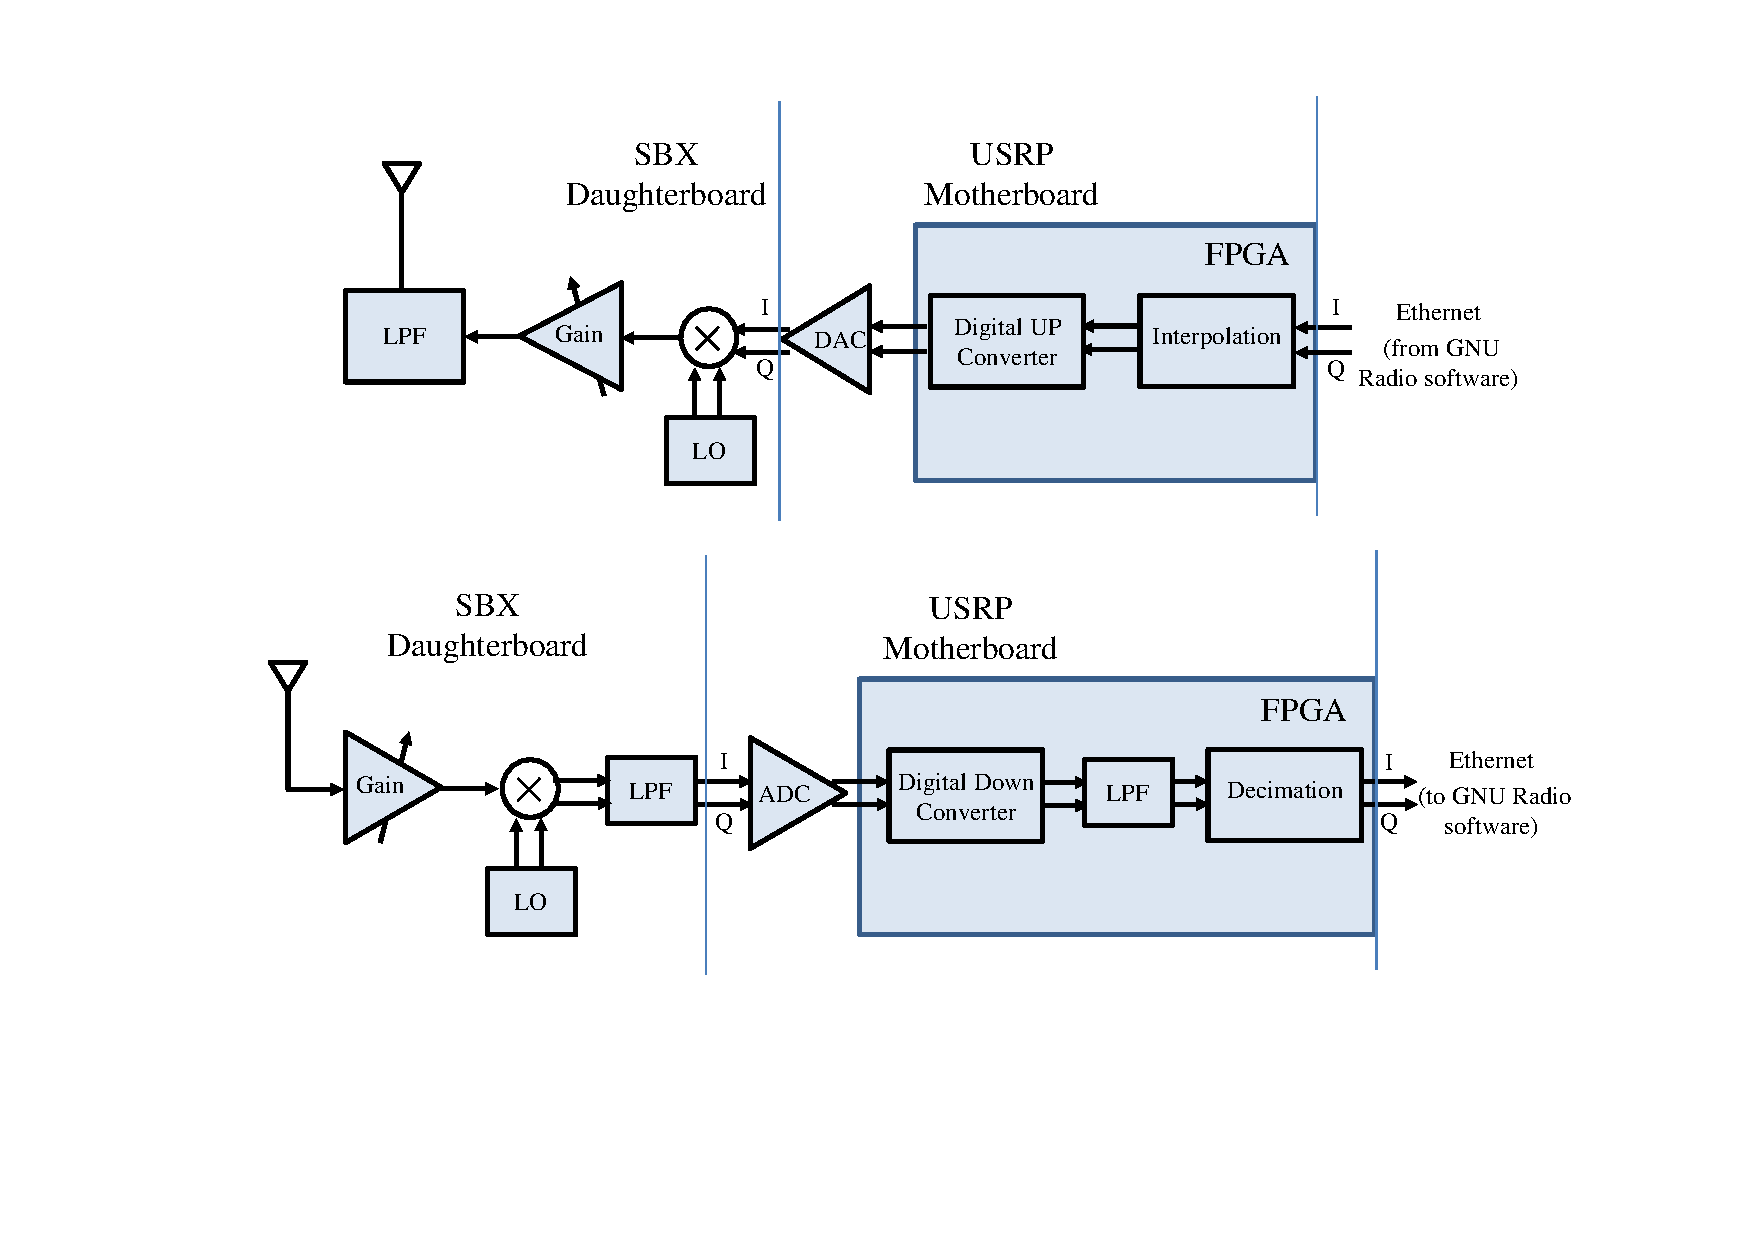
\includegraphics[width=180mm]{USRPandSBX.pdf}}
    \caption{Block diagram of the key components on the USRP N210 motherboard and the SBX daughter board.}
    \label{fig:USRPandSBX}
  \end{center}
\end{figure}


Figure~\ref{fig:USRPandSBX} shows the structure of the USRP N210 mother board and SBX daughter board. Ethernet connects the USRP to a computer running a GNU Radio program.


\section{The Spectrum Challenge}
Radios can often interfere with other radios and disrupt the operations. The DARPA Spectrum Challenge is a competition initiated in January 2013 to demonstrate a radio protocol that can best use a given communication channel in the presence of other dynamic users and interfering signals. The Challenge focuses on finding strategies instead of developing new radio hardware to guarantee robust wireless communication in congested electromagnetic environments \cite{DARPASpectrumChallenge}.

There are also other factors that motivate the need for distributed spectrum sharing. In rapid response operations, such as disaster relief, multiple radios come to the same geographic region and may try to use the same spectrum. It is desirable for the radios to efficiently share the spectrum without prior coordination. In the military and civilian sectors, high priority radios are required to operate regardless of the electromagnetic interference, to guarantee reliable communications and to avoid potential loss of life. Corresponding to these two needs, two matches were created in the Challenge: the cooperative match and the competitive match. Eighteen teams competed in the competitive match and the cooperative match in the Final Tournament.

\subsection{Challenge Rules}

The Spectrum Challenge uses the ORBIT test bed for design development, practice sessions, and tournaments \cite{OrbitLab}. It has implemented a SDR platform consisting of computers and USRP N210s. Teams may use any software development tools and programming languages, but no modifications of the test bed hardware is permitted. The final design must run on the ORBIT test bed by simply loading an image and executing a single console command.

All radios must be designed to operate within a limited bandwidth. The allowable bandwidth is controlled by two parameters: the specified RF center frequency of the band, denoted $F_c$, and the maximum sampling rate of the USRP, denoted $R_{max}$. In the Final Challenge event, $F_c=600$ MHz, and $R_{max}=5$ million samples per second for both the transmitter and receiver. The allowable frequency band is therefore given by
\begin{align}
F_c - R_{max}/2 \le f \le F_c + R_{max}/2.
\end{align}
This constraint does not imply that the radio's carrier frequency must be set to be $F_c$, nor does it require the sampling rate to be $R_{max}$ at all times. However, the allowable bandwidth for the transmitter and receiver is restricted by the maximum sample rate and the specified center frequency $f$ by
\begin{align}
&f+\frac{r}{2} \le F_c + R_{max}/2&\\
&f-\frac{r}{2} \ge F_c - R_{max}/2,&
\end{align}
where $r$ is the user-programmed sampling rate. The radio could transmit anywhere within the actual bandwidth limitation as long as the chosen carrier frequency and sampling rate satisfy the above limits.

The total transmission power is not limited, but it is restricted by the hardware, USRP N210. Since every team uses the same type of hardware, the maximum achievable transmission power can be assumed to be the same for each team. The actual transmission power of each team depends on their radio design.

In both competitive and cooperative games, one radio node in each pair draws packets from the server and the other delivers packets back to the server. Drawn and delivered packet sizes are fixed at 1440 bytes and the total file size, i.e., total number of packets ($D$) is 15000.

\subsubsection{Radio Geometry and ORBIT Grid Configuration}
Figure~\ref{fig:CooperativeNodeAssignement} shows the radio node geometry for the cooperative match. There are three teams in each cooperative game. The source and destination nodes are labeled by S and D, respectively. The source node requests data packets from the server, and the destination node returns data packets to the server. The goal is to transmit data packets from the source to the destination.

The distance $R_1$ from the source to destination is roughly 76 feet, and the distances $R_2$ between source nodes (S1-S3 and S2-S3 ) and between destination nodes (D1-D3 and D2-D3) is roughly 3 feet.

\begin{figure}[tpb]
  \begin{center}
    \centerline{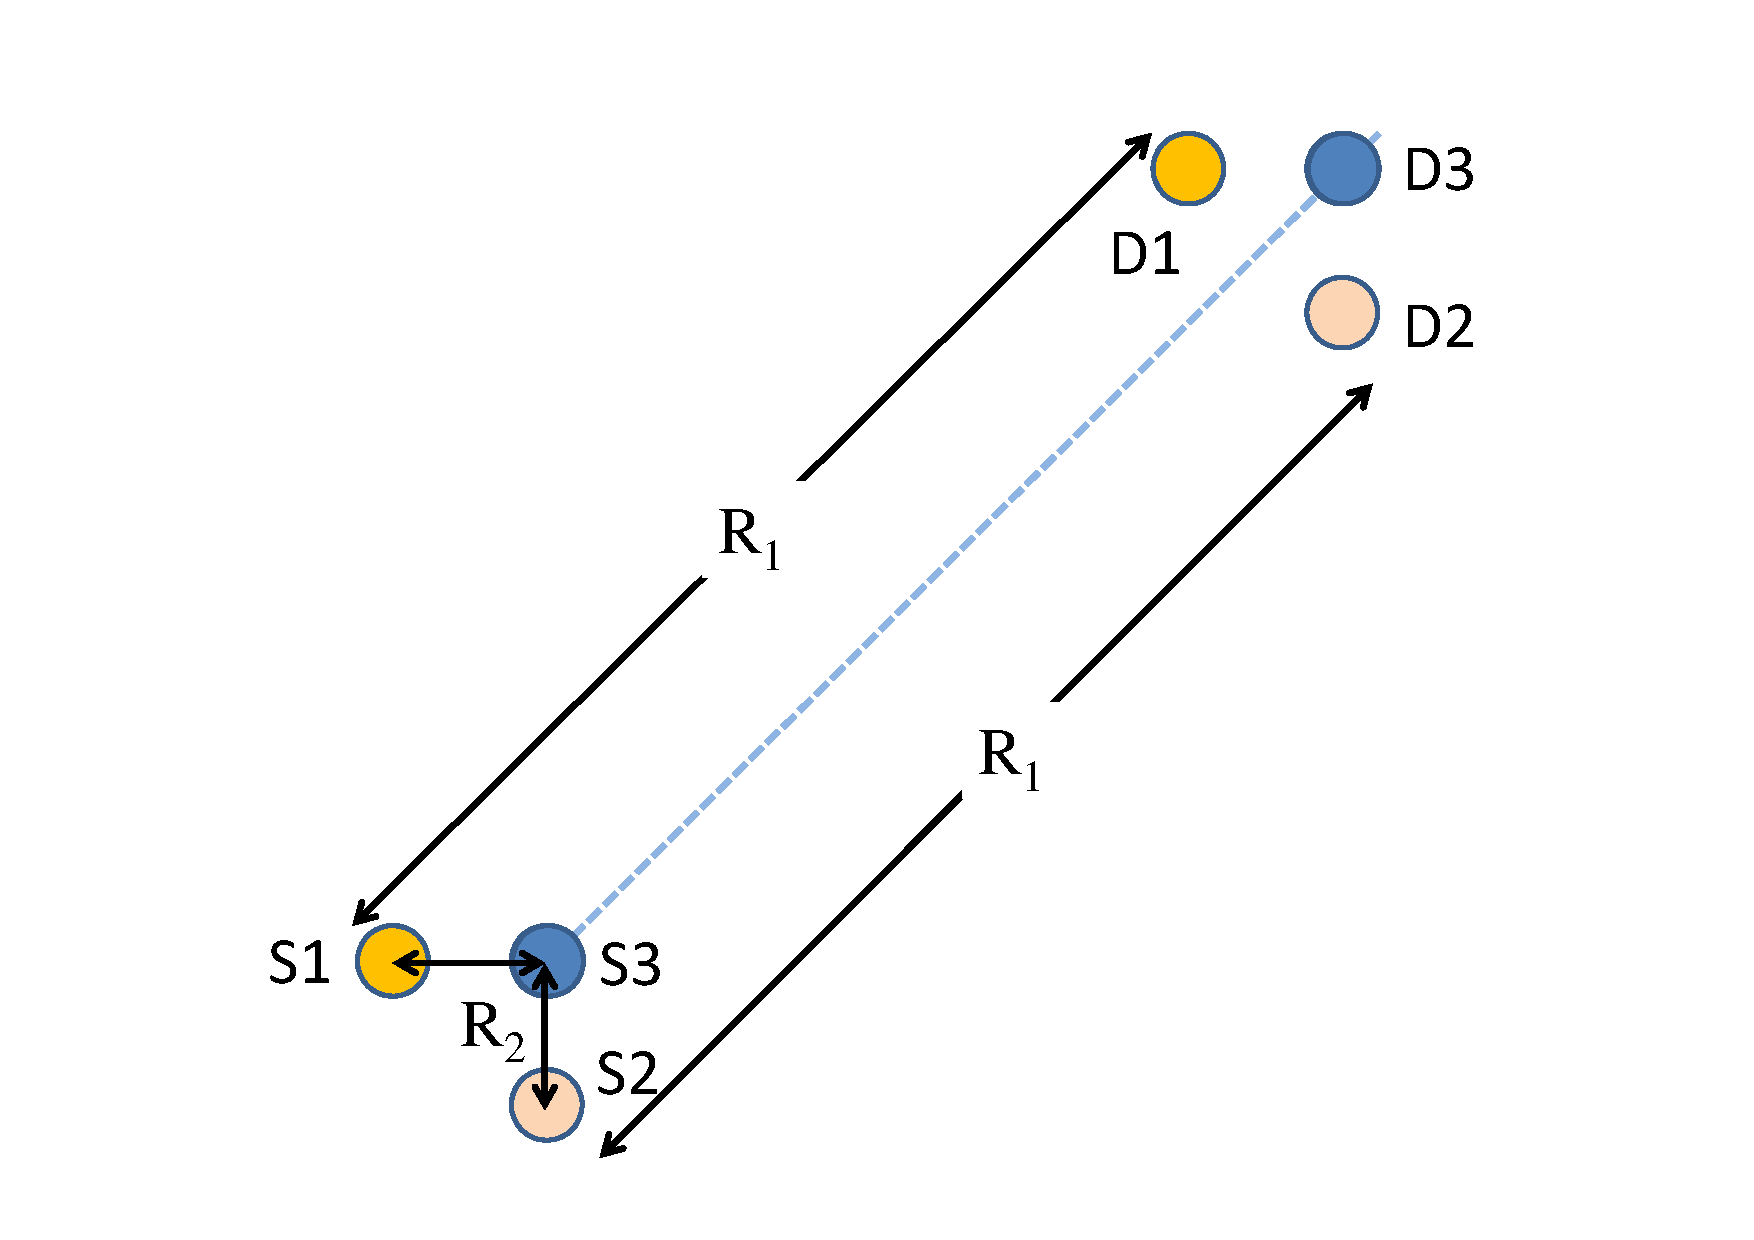
\includegraphics[width=150mm]{CooperativeNodeAssignement.pdf}}
    \caption{Radio node geometry for the cooperative match. The distances are roughly $R_1=76$ feet and $R_2=3$ feet.}
    \label{fig:CooperativeNodeAssignement}
  \end{center}
\end{figure}

Figure~\ref{fig:CompetitiveNodeGeometryFinalRound} shows the radio node geometry for the competitive match. There are two teams competing with each other in each competitive game and they are represented by different colors. The distances $R$ R between nodes in the pairs S1-D1, S2-D2 and D1-D2 is roughly $R=$ 25 feet.
\begin{figure}[tpb]
  \begin{center}
    \centerline{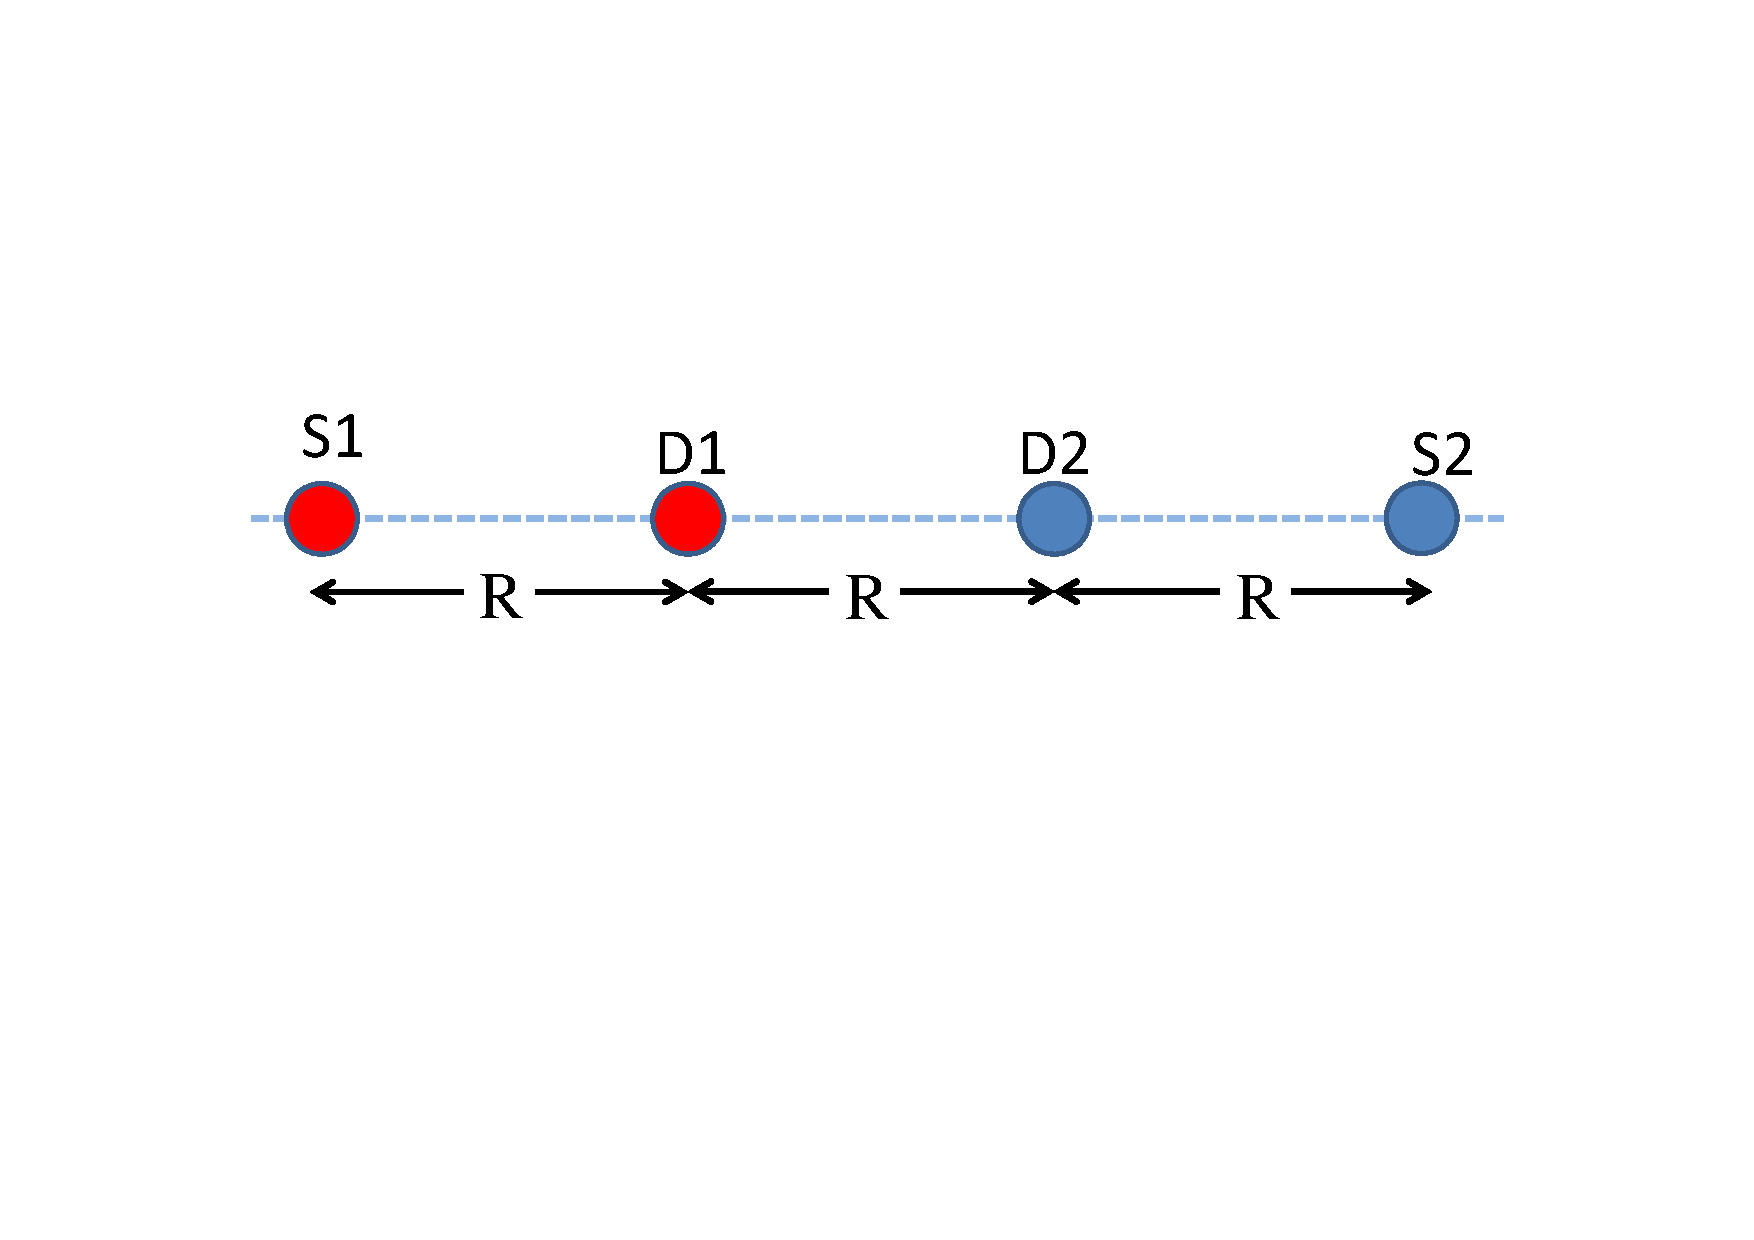
\includegraphics[width=150mm]{CompetitiveNodeGeometryFinalRound.pdf}}
    \caption{Radio node geometry for competitive match. The distances are roughly $R=25$ feet.}
    \label{fig:CompetitiveNodeGeometryFinalRound}
  \end{center}
\end{figure}

A match consists of two games such that a team plays one game using the S1/D1 pair and the other game using the S2/D2 pair. Each team's score for a match is the sum of its successful packets transferred in both games.

\subsection{Cooperative Tournament}
The tournament structure consisting of a number of matches among three teams is depicted in Figure~\ref{fig:CooperativeTournamentStructure}. The three rounds are the preliminary round, semifinal round and final round. The score of each team in one round is not counted in other rounds.

\begin{figure}[tpb]
  \begin{center}
    \centerline{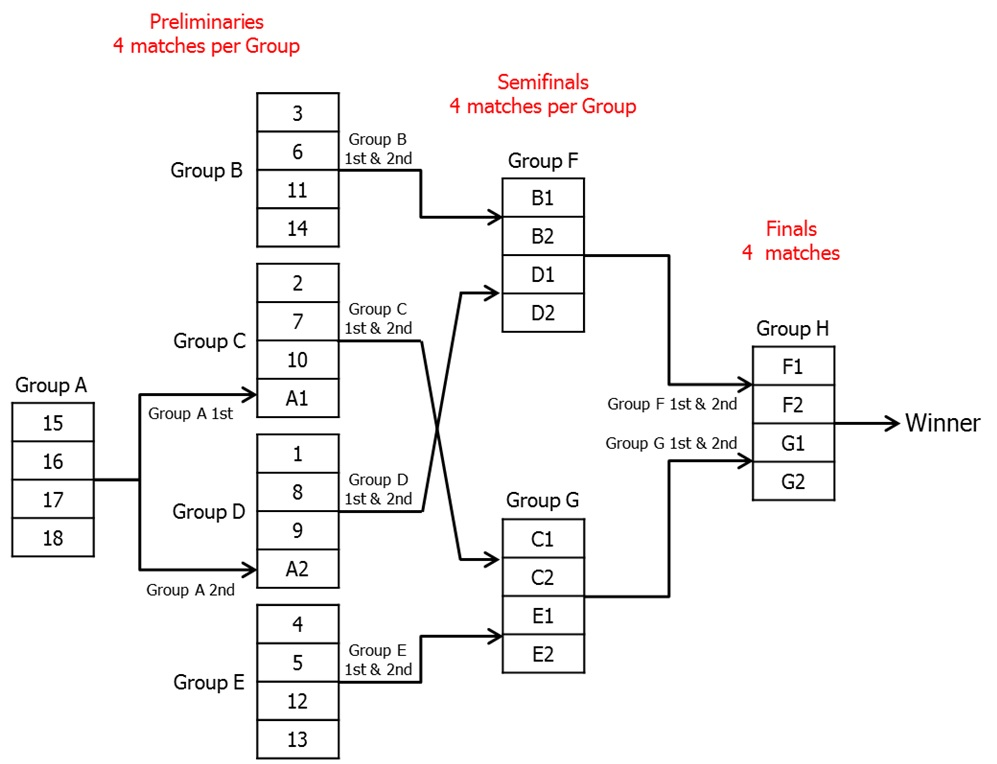
\includegraphics[width=170mm]{CooperativeTournamentStructure.jpg}}
    \caption{Cooperative Tournament Structure}
    \label{fig:CooperativeTournamentStructure}
  \end{center}
\end{figure}

The cooperative game ends (at time $t$) once all three radio pairs have successfully transmitted all of their data or once the maximum time ($T = 3$) minutes is reached. Suppose that $X_i$ ($i=1,2,3$) denotes the number of packets successfully transferred for team $i$. Sort $X_i$ in descending order to get $Y_1$, $Y_2$ and $Y_3$. The score for team $i$ is
\begin{align}
{S_i} = {X_i} + {Y_1} + {Y_2}, \quad i=1,2,3.
\end{align}
This scoring scheme encourages each team to be aggressive in the cooperative game.

In the preliminary round, 18 teams are divided into 5 groups of 4 (Groups A to E). One spot in each of Groups C and D is filled with the top two teams from Group A. Within each group, games are played among all combinations of 3 teams, resulting in 3 games per team. A team's match score is the sum of its 3 game scores in the current round. The 2 teams with the highest match scores from Groups B and C advance to the semifinal round as Group F. The 2 teams with the highest match score from Groups D and E advance as Group G.

In the semifinal round, the 2 groups of 4 teams (Groups F and G) play all combinations of 3 teams, with three games in each match to average out radio configurations as in earlier rounds, and each team accumulates a match score from its 3 games. The first and second highest scoring teams from each group advance to the final round.

In the final round, the 4 remaining teams play in all combinations of 4 and accumulate a score from their 4 matches. The winner is the team with the highest match score in the final round.


\subsection{Competitive Tournament}
The tournament structure is depicted in Figure~\ref{fig:CompetitiveTournamentStructure}. The three rounds are the preliminary round, semifinal round and final round. The score of each team in one round is not counted in other rounds.
\begin{figure}[tpb]
  \begin{center}
    \centerline{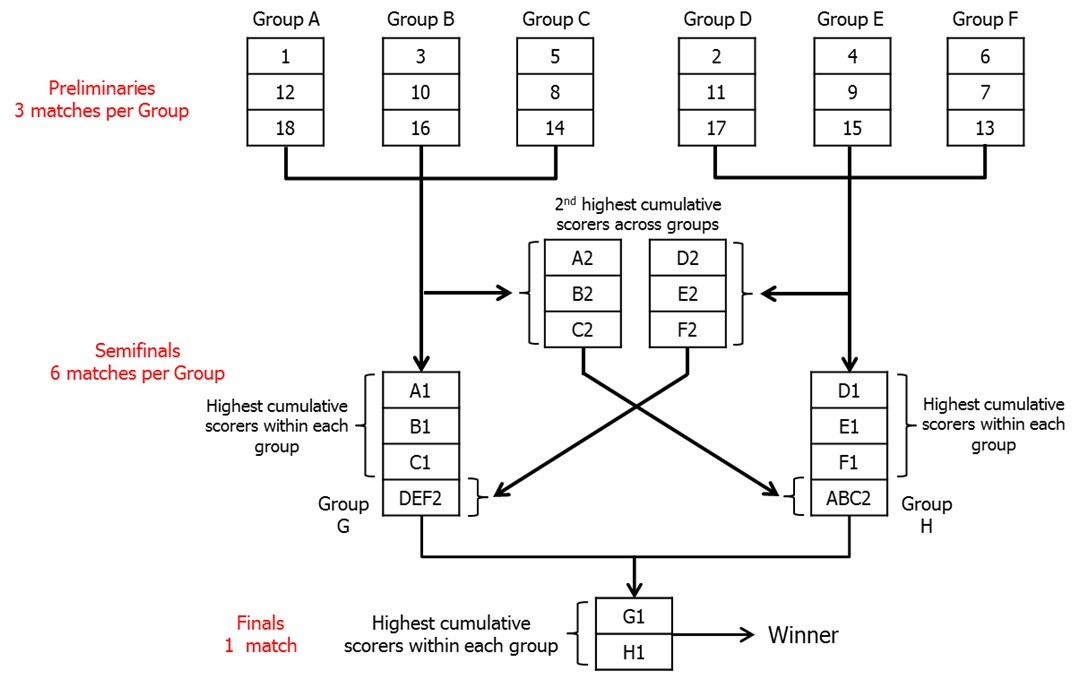
\includegraphics[width=170mm]{CompetitiveTournamentStructure.jpg}}
    \caption{Competitive Tournament Structure}
    \label{fig:CompetitiveTournamentStructure}
  \end{center}
\end{figure}

In the preliminary round, the 18 teams are divided into 6 groups of 3 (Group A to F). Within each group, matches are played between all pairs of teams, providing 2 games per team. A team's match score is the sum of the 2 game scores, i.e., the total number of packets successfully transferred. In a game, a team completes a trial using the S1/D1 nodes and another trial using the S2/D2 nodes. The team with the highest match scores across the games played within each group advances to the semifinals. The teams with the second highest scores in Group A, B, and C are designated A2, B2, and C2 in Figure~\ref{fig:CompetitiveTournamentStructure}. Teams A2, B2, and C2 play all combinations (2 games per team), and the team with the highest cumulative score advances to the semifinals as team ABC2. Similarly, the teams with the second highest scores in Groups D, E, and F(D2, E2, and F2) play all combinations and the team with the highest cumulative score advance as team DEF2

In the semifinal round, the 2 groups of 4 teams (Groups G and H) play all combinations. Each team accumulates a score from its 6 games. The teams with the highest scores within each group advance to the final round.

The final round consists of 1 match, again of two trials to account for radio variations, to determine the overall winner.

\section{Preliminary Analysis}
Preliminary analysis is conducted based on the radio geometries and game metrics. Many of these aspects will be discussed and designed in details in later chapters.
\subsection{Preliminary Cooperative Analysis}
Our radio should avoid conflicting with other teams in frequency. In the Spectrum Challenge, no spectrum usage of other radios is disclosed in advance. Therefore, spectrum sensing is necessary to analyze the spectrum usage of other teams. From Figure \ref{fig:CooperativeNodeAssignement}, the sources are crowded together, which means that most of the signal energy from each radio is on the source side. As a result, the spectrum sensing should be done on the source side.

The reverse link (from destination to source) has low signal-to-interference ratio (SIR), and feedback seems to be impossible. However, if a narrow-band signal is used, the SIR can be significantly increased in that narrow band. Tests have demonstrated narrow-band feedback is achievable if the feedback signal is transmitted on the channel where no interference from other teams is present on the source side.

\subsection{Preliminary Competitive Analysis}
A good power control strategy for each team in the competitive game is to spread the available power over the entire bandwidth using the water filling method. Since equilibrium strategy for each team is to spread power evenly across the entire spectrum as discussed in \cite{REtkinandAParekhandDTse2007}, the strategy implemented in our radio should include such strategy.

From Figure~\ref{fig:CompetitiveNodeGeometryFinalRound}, the reverse link should have lower SIR than the forward link, and should be more reliable than the forward link. Therefore, feedback can be implemented to increase the throughput.

\section{Physical-Layer Foundation}
Orthogonal frequency-division multiplexing (OFDM) is used as the core modulation technique in our radio \cite{DingNieCompetitivePlan2013}. OFDM is chosen for several reasons. First the symbol rate can correspond to the maximum sampling rate of 5 MHz, whereas single-carrier modulation techniques require excess bandwidth and over-sampling. Second, OFDM is more flexible with multiple tones that can be used or not, which is significant in our competitive and cooperative strategies.

For both the cooperative radio and competitive radios, 512 tones are used, each with 9.77 kHz subcarrier spacing. We index the tones as tone $1,2,3,...,512$, from the lowest frequency to the highest frequency. A cyclic prefix (CP) with length of 8 samples is used in one OFDM symbol to allow for low-complexity estimation and equalization of multipath fading. The length for each OFDM symbol is 520 samples, or 104 $\mu s$.

We now highlight differences between the physical-layers of the cooperative radio and the competitive radio.

\subsection{Physical Layer Specification of the Cooperative Radio}
\label{coopPhysicalLayer}
An OFDM sub-frame consists of 1 symbol of preamble followed by 16 OFDM data symbols for a total of 17 OFDM symbols. The preamble is used to enable time and frequency synchronization as well as channel estimation at the receivers. In the frequency domain, the preamble is a set of pseudo-random sequences of -1, 0 and +1 known to both the source and destination, and the non-zero values appear every 8 tones except for the DC tone. The 512 OFDM tones are divided into 16 sub-bands as shown in Figure~\ref{fig:CoopPhysicalLayer}. Tones 1 to 13, tones 254 to 259 and tones 500 to 512 are not used because of the rolloff effect on the edge of 5 MHz and because of the DC offset around the DC tone. The unused tones correspond to a sort of 6.7$\%$ excess bandwidth. All the remaining 480 tones are divided evenly into 16 sub-bands and each sub-band has 30 tones. We index the sub-band as sub-band $1,2,...,16$ from lowest to highest frequencies. Each sub-band can be turned on and off separately, including the preamble in that sub-band.

In the time domain, the preamble symbol has 8.125 identical repetitions during 104$\mu s$. This repetition feature helps the receiver to identify the preamble and acquire OFDM synchronization. In the cooperative radio, preambles are also used as pilots to do channel estimation in the 5 MHz bandwidth. In the frequency domain, the non-zero symbols are placed every 8 tones. Based upon measurements using the ORBIT testbed, the channel appears quite flat, so averaging can be performed across frequency when estimating the channel.

\begin{figure}[tpb]
  \begin{center}
    \centerline{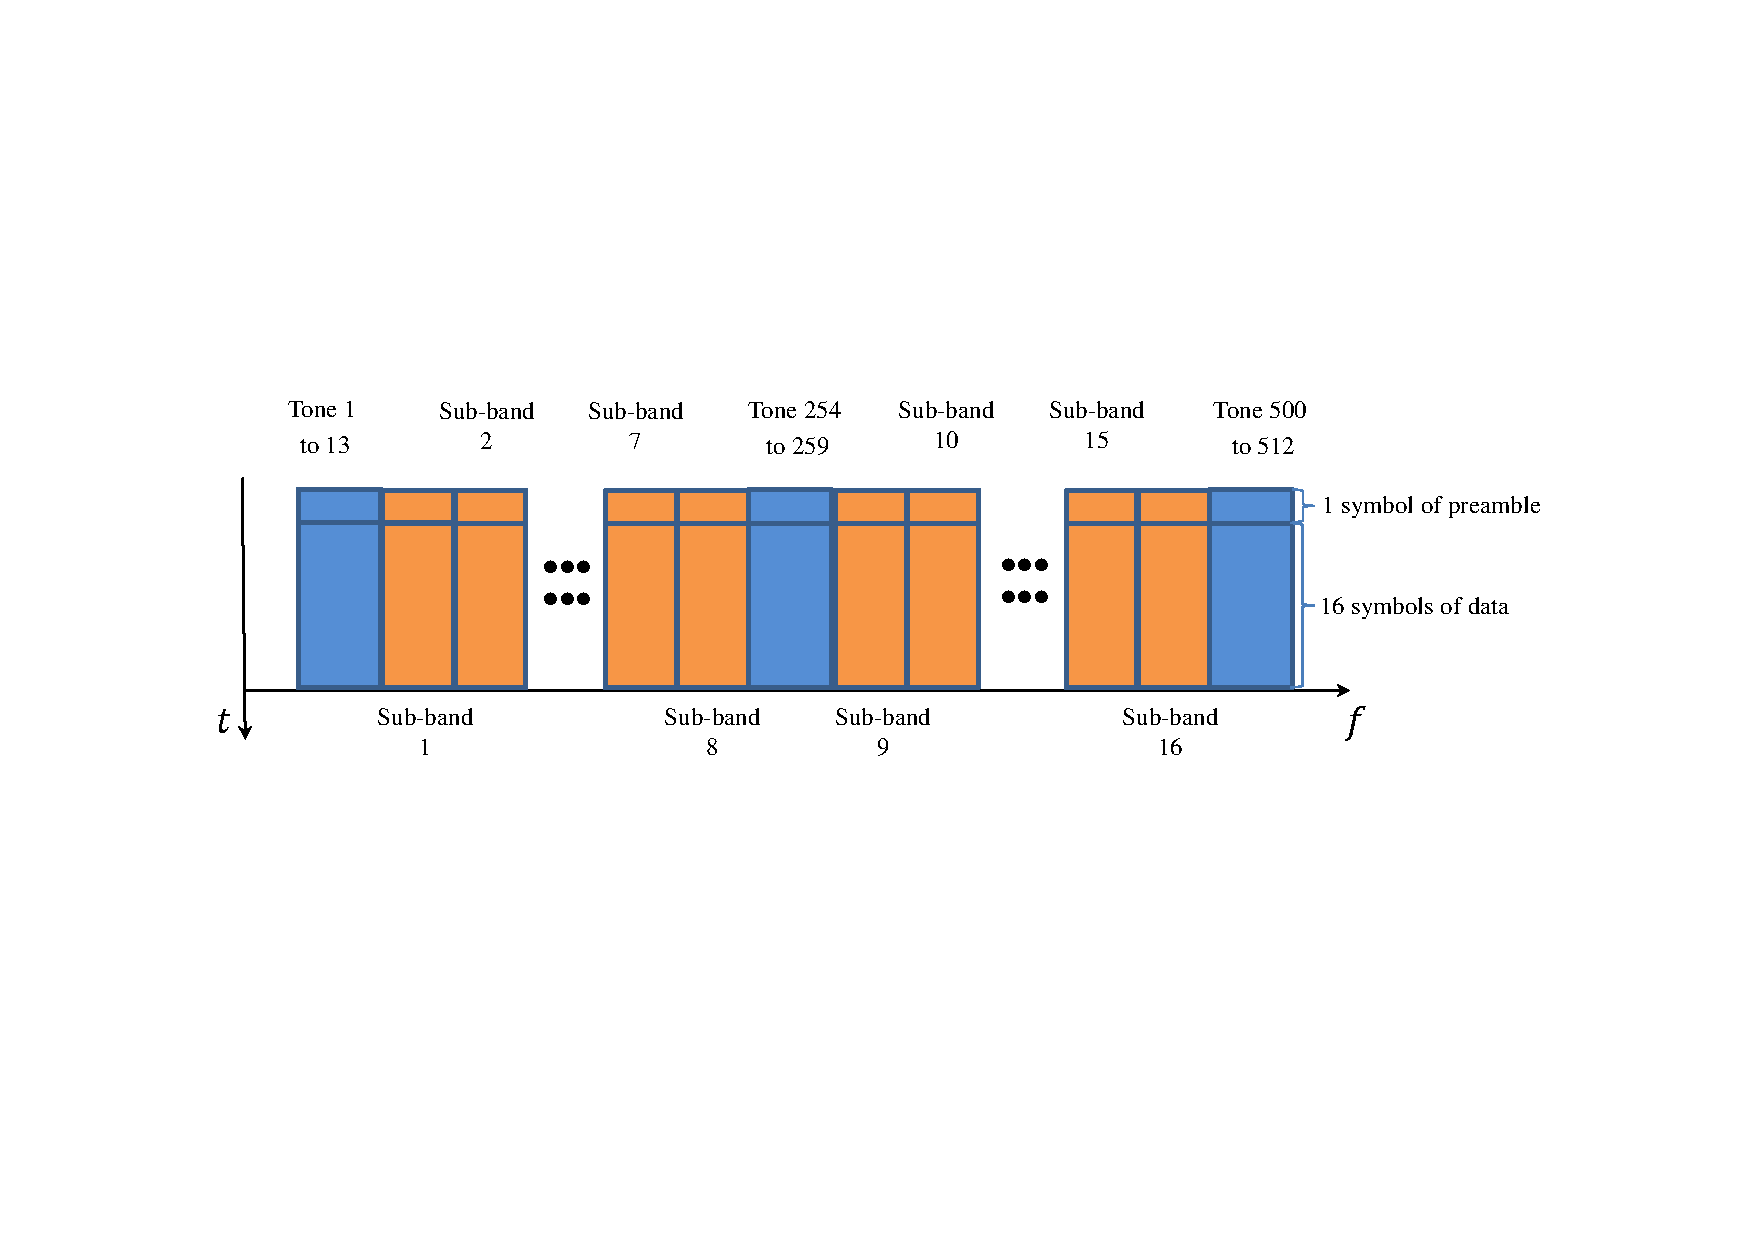
\includegraphics[width=160mm]{CoopPhysicalLayer.pdf}}
    \caption{OFDM specifications for the cooperative radio. The darker color indicates unused sub-bands, and the lighter color indicates used sub-bands.}
    \label{fig:CoopPhysicalLayer}
  \end{center}
\end{figure}

\subsection{Physical Layer Specification of the Competitive Radio}
An OFDM sub-frame consists of 1 symbol of preamble followed by 1 symbol of pilot and 16 OFDM data symbols for a total of 18 OFDM symbols. In the frequency domain, the non-zero values of the preamble appear every 2 tones except for the DC tone, and the non-zero values of pilot are placed every 8 tones except for the DC tone. The 512 OFDM tones are divided into 8 sub-bands as shown in Figure~\ref{fig:CompPhysicalLayer}. Tones 1 to 13, tones 254 to 259 and tones 500 to 512 are not used similar to the cooperative radio. All the remaining 480 tones are divided evenly into 8 sub-bands, with each sub-band having 60 tones. We index the sub-band as sub-bands $1,2,...,8$ from lowest to highest frequencies. The data OFDM symbols of each sub-band can be turned on and off separately, but the preamble and pilot symbols are always generated.

\begin{figure}[tpb]
  \begin{center}
    \centerline{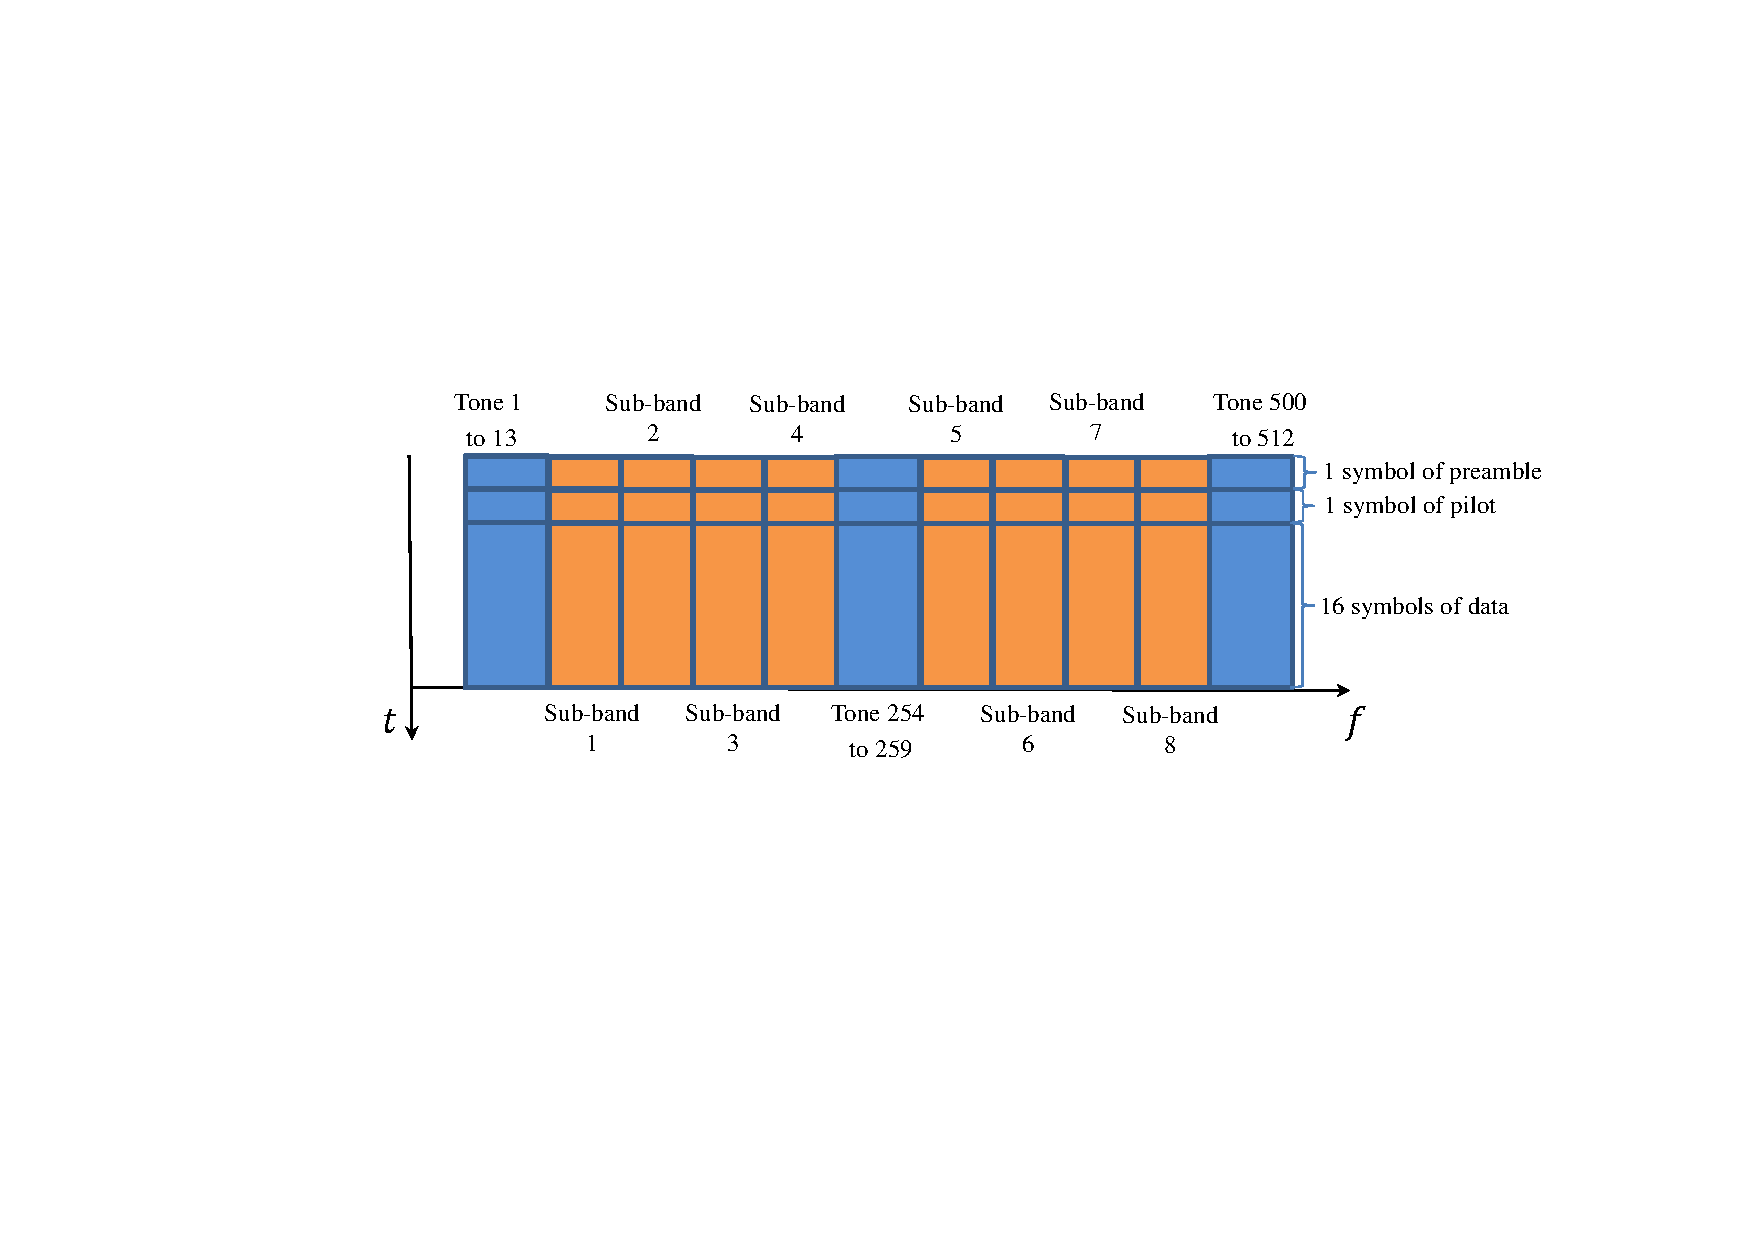
\includegraphics[width=160mm]{CompPhysicalLayer.pdf}}
    \caption{OFDM specifications for the competitive radio. The darker color indicates unused sub-bands, and the lighter color indicates used sub-bands.}
    \label{fig:CompPhysicalLayer}
  \end{center}
\end{figure}
